
\begin{frame}[t]\frametitle{Qué es una palabra contrastiva}
    
    Se dice que una palabra es \textit{contrastiva} cuando la frecuencia de uso en distintas regiones es muy diferente. 

    \begin{block}{Ejemplos palabras contrastivas Argentina - España}
    \begin{itemize}
        \item ``che''
        \item ``metegol''
    \end{itemize}
    \end{block}

    \begin{block}{Ejemplos palabras contrastivas dentro de Argentina}
    \begin{itemize}
        \item ``gurisada''
    \end{itemize}
    \end{block}

    ¿Para qué sirve conocer las palabras contrastivas?

\end{frame}

\begin{frame}[t]\frametitle{Léxico contrastivo}
    \centering{Palabra:Manso}
     
     \begin{columns}[t]  
        \begin{column}{.48\textwidth}
            \begin{figure}
                
\includegraphics[width=0.95\textwidth]{../src/images/presentacion/mendoza.png}
                \caption{Frecuencia de uso en {Mendoza}}
                \label{fig:mendoza}
            \end{figure}
        \end{column}
        % \hfill
        \begin{column}{.48\textwidth}   
            \begin{figure}
                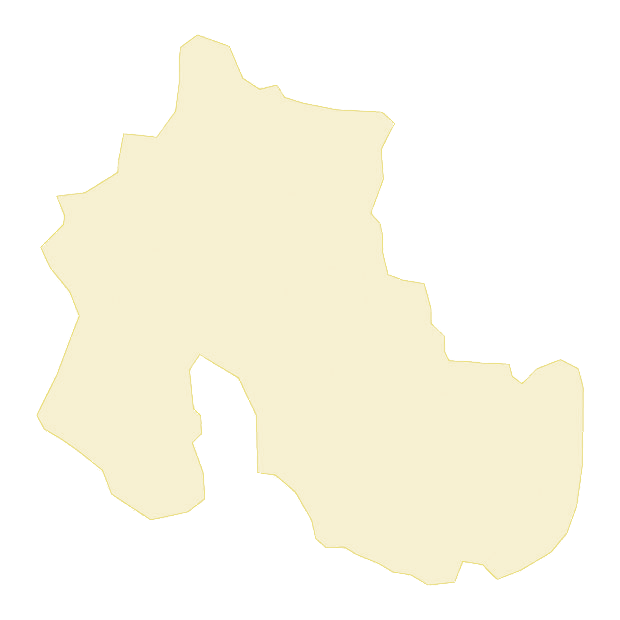
\includegraphics[width=0.95\textwidth]{../src/images/presentacion/jujuy.png}
                \caption{Frecuencia de uso en {Jujuy}}
                \label{fig:jujuy}
            \end{figure} 
        \end{column}
    \end{columns}

\end{frame}

\begin{frame}[t]\frametitle{Motivación de un método computacional para detectar léxico contrastivo}
    
    ¿Cómo se conocían las palabras contrastivas?
    \textbf{Mediante encuestas.}
    \begin{itemize}
        \item Costosas de realizar
        \item Muy difícil de hacer de forma balanceada en distintas regiones de un país o de un continente.
        \item Más difícil aún es encuestar a una gran cantidad de personas.
        \item \alert{Se basan en el conocimiento \textit{a priori}}
    \end{itemize}
\end{frame}